\documentclass[conference]{IEEEtran}
\usepackage[ngerman]{babel}
\usepackage[utf8]{inputenc}
\usepackage[T1]{fontenc}
\usepackage{graphicx}
\usepackage{caption}
\usepackage{subcaption}

\begin{document}
\title{Verteilte eingebettete Systeme für Netzwerk-Service-Assurance-Tests}
\author{\IEEEauthorblockN{Christian Rebischke}
\IEEEauthorblockA{Technische Universität Clausthal\\
Rechenzentrum\\
Email: Christian.Rebischke@tu-clausthal.de}}

\maketitle

\begin{abstract}
    Um eine gleichbleibende Netzqualität innerhalb des Netzes der
    TU-Clausthal zu gewährleisten werden Einplatinen-Computer auf dem
    Campus verteilt um Service-Assurance-Tests durchzuführen. Diese
    Tests sollen eine gleichbleibende und stabile Verbindung garantieren
    und bei Abweichen von Mess-Ergebnissen einen Netzwerk-Administrator
    alarmieren. Die Ergebnisse sollen in einer Datenbank gespeichert und
    entsprechend für die weitere Verwertung gefiltert und aufgewertet
    werden. Dabei ist geplant die Masse an Einplatinen-Rechnern mit
    State of the Art Orchestration und Config Management Tools im
    Schwarm zu administrieren. Zusätzlich ist es denkbar über diese
    verteilten Netzwerk-Knoten diverse Sicherheits-Tests im Netzwerk
    durchzuführen wie beispielsweise das Erkennen von ungewünschten
    WLAN-Hotspots oder von Angreifern innerhalb des TU-Netzes.
\end{abstract}

\IEEEpeerreviewmaketitle

\section{Einleitung}
Im Zeitalter immer stärkerer Digitalisierung bekommt ein stabiles und
zuverlässiges Netz eine immer wichtigere Rolle. Dies spürt man gerade im
akademischen Umfeld in dem Themen wie verteiltes Rechnen eine große
Rolle spielt. Abweichungen oder Netzausfälle können in so einem Fall
ganze Berechnungen zu nichte machen. Um solch ein stabiles Netz zu
gewährleisten gibt es Service-Assurance-Tests. Service-Assurance-Tests
sollen eine bestimmte Service-Qualität versichern. Dies kann anfangen
bei einer Uptime-Garantie, über eine Bandbreiten-Garantie bis zur
Überwachung von Service-Level-Agreements.
\subsection{Technische Details}
Als Grundlage für die Service-Assurance-Tests sollen
Einplatinen-Computer wie beispielsweise der Raspberry Pi oder der Odroid
dienen. Der Vorteil davon ist ein geringer Preis in der Anschaffung und
eine stabile Basis auf offener Software die es ermöglicht das System
beliebig zu erweitern und zu verändern. Als Betriebssystem wird eine auf
Debian oder CentOS basierte Linux-Distribution zum Einsatz kommen. Um
maximale Genauigkeit zu garantieren ist außerdem ein nativer
1Gigabit-Ethernet-Port von nöten. Die restlichen Hardware-Anforderungen
sind variabel, aber 20GB Festplatte in Form eines Flash-Speichers, bis
zu 4 CPU Kerne und 2-4GB RAM sollten ausreichen. Um die veteilten
Einplatinen-Rechner zentral zu verwalten ist ein modernes
Configuration-Management mit einer Key-Value-Datenbank in Form von Hiera
und Puppet geplant. Dafür wird es einen zentralen Puppet-Server geben
von dem aktuelle Konfigurationsdaten mit einem Pull-Mechanismus an die
Clients verteilt werden. Dadurch ist manuelles Arbeiten auf den Clients
nicht mehr nötig. Die von den Clients gewonnenen Daten sollen an eine
zentrale Datenbank weitergeleitet werden. Zur Visualisierung ist eine
Grafana-Instanz geplant.
\begin{figure}[h]
    \centering
    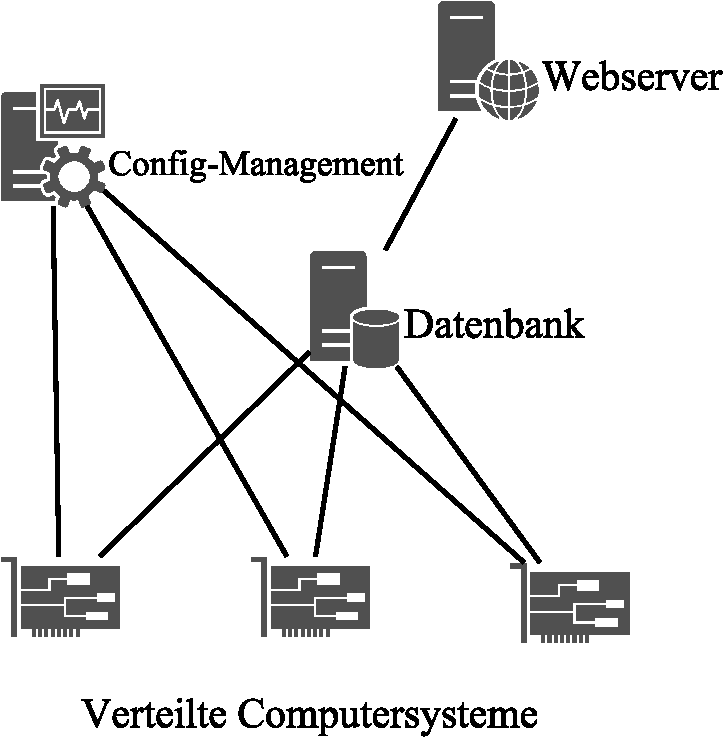
\includegraphics[width=0.5\textwidth]{figures/network.pdf}
    \caption{Netzwerk-Grundriss des Projekts}\label{fig:1}
\end{figure}

\section*{Danksagung}
Ich danke dem Rechenzentrum der TU-Clausthal, dass ich dort meine
Bachelor-Arbeit schreiben darf.

\end{document}
